\chapter{化学家的量子力学：模型体系}\label{ch:b3:quantum-model-systems}

实验台上放着三只小烧瓶，各盛一种花青染料的乙醇溶液：
第一只呈品红色，第二只呈蓝色，第三只呈深绿蓝色，
在远红光区有吸收。三个分子结构相似——
两端是两个相同的含氮环，由一段碳链相连——
三者只在链长上有所不同，每次相差两个碳原子。
碳链越长，颜色越向红端移动。
1949 年，一位化学家用量子力学中最简单的问题之一解释了这一系列现象：
一个电子在长度固定的直线上自由运动，
即“箱中粒子”。本章建立该解释所依托的理论工具——
算符、本征值与薛定谔方程——并
求解化学中日常使用的模型体系：箱中粒子、
振动化学键的谐振子、转动分子的刚性转子、
氢原子，以及轻粒子能够穿过的势垒，
即使其能量不足以翻越该势垒。

\begin{recall}
本科一年级分册表明，原子的能量是量子化的（能级、基态与激发态、氢原子光谱线），并且
光子所携带的能量为
$E = h\nu = hc/\lambda$。本科二年级分册以波函数描述电子，
波函数 $\psi$ 的平方为概率密度，并将氢原子轨道分为径向部分与角向部分，
并数出它们的节点；
当时直接取氢原子波函数为已知；此处在第 5 节给出推导。
取自物理学的内容有：动量 $p = mv$，以及德布罗意波长
$\lambda = h/p$。
\end{recall}

\begin{omfigure}
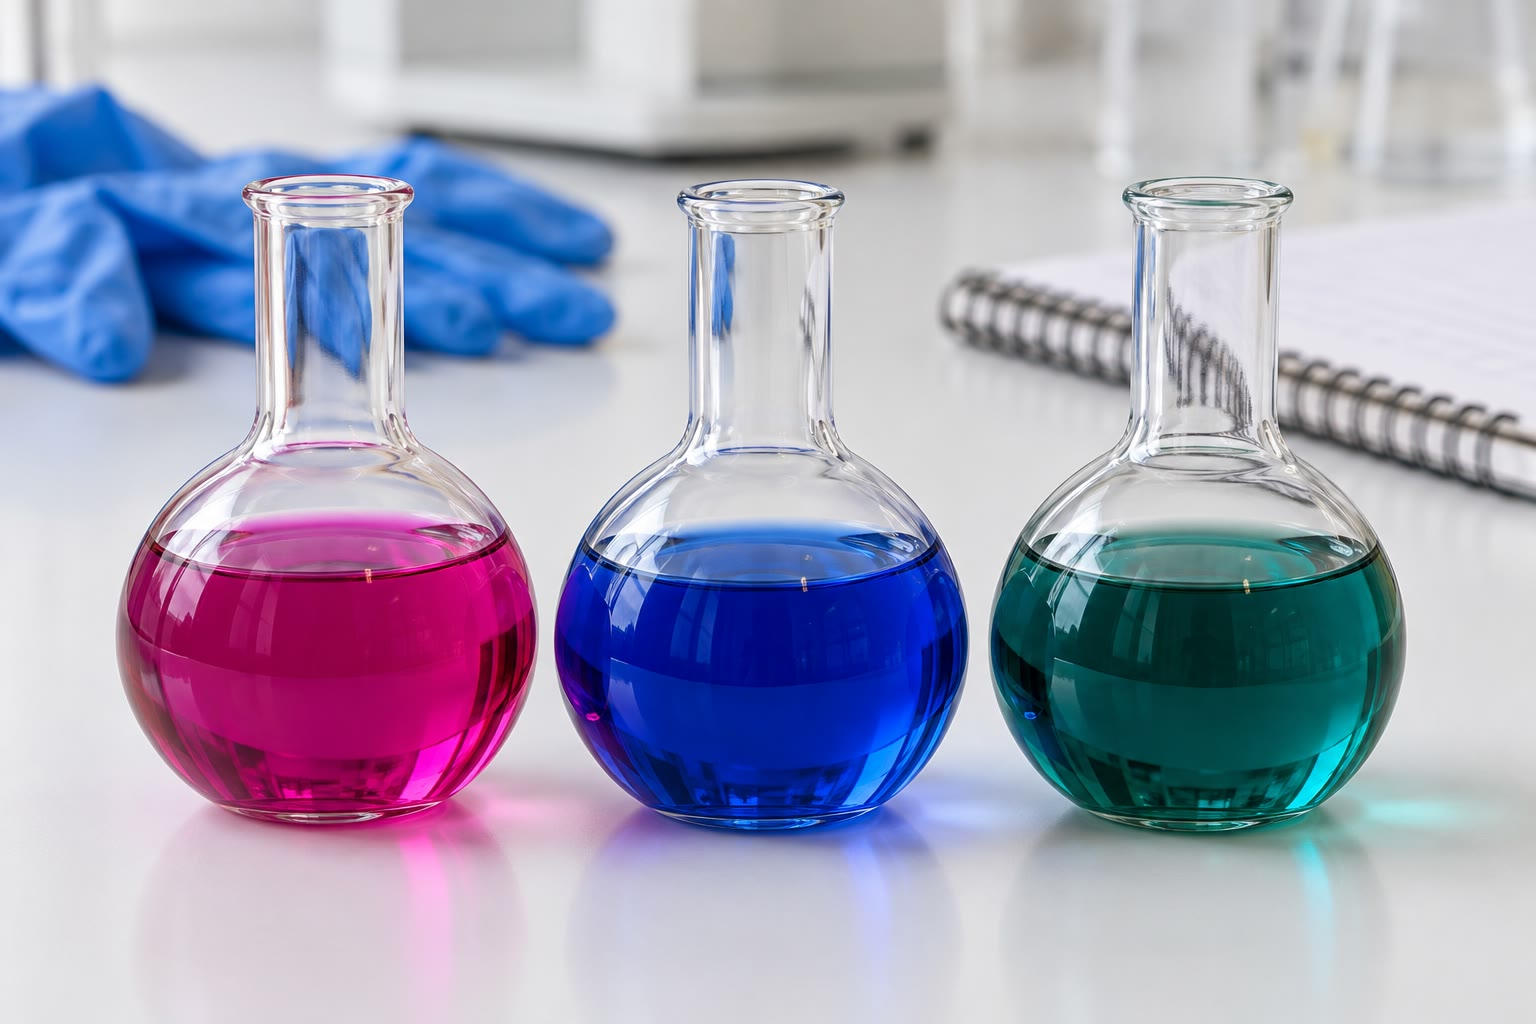
\includegraphics[width=0.62\linewidth]{images/book4/ai/b3-01-dyes.jpg}

{\small 同一家族的三种花青染料溶液。链中每增加
一对碳原子，吸收峰便向红端移动。}
\end{omfigure}

\section{算符、本征值与薛定谔方程}

经典力学在每一时刻给出粒子的位置与动量。
量子力学则给出粒子的状态，即波函数 $\psi$，
并用作用于 $\psi$ 的运算替代每一个可测物理量。

\begin{definition}[算符、本征函数、本征值]\label{def:b3:quantum-model-systems:operator}
称 $\hat A$ 为\emph{算符}\index{算符}，它是把一个函数
变为另一个函数的规则：$\hat A f = g$。若 $\hat A(\lambda f +
\mu g) = \lambda\hat Af + \mu\hat Ag$，则它是线性的。若非零函数 $f$ 满足
$\hat Af = a f$，其中 $a$ 为某个数，则该函数称为
$\hat A$ 的\emph{本征函数}\index{本征函数}，$a$ 称为相应的\emph{本征值}\index{本征值}。
\end{definition}

\begin{example}[位置与动量的两个算符]\label{ex:b3:quantum-model-systems:xp}
在一维情形下，位置算符是乘以 $x$：$\hat x f = xf$，
动量算符则是求导：$\hat p f = -\iu\hbar\,
\dd f/\dd x$，其中 $\hbar = h/2\pi$。函数 $\eu^{\iu kx}$ 是
$\hat p$ 的本征函数，本征值为 $\hbar k$：波长为
$\lambda = 2\pi/k$ 的波具有动量 $h/\lambda$，这正是德布罗意关系。
函数 $\sin kx$ 不是 $\hat p$ 的本征函数（其导数为
余弦函数），但它是 $\hat p^2 = -\hbar^2\,\dd^2/\dd x^2$ 的本征函数，
本征值为 $\hbar^2k^2$。
\end{example}

\begin{definition}[厄米算符、期望值]\label{def:b3:quantum-model-systems:hermitian}
记 $\langle f|g\rangle = \int f^*g\,\dd\tau$，两函数在区域边界上为零。
若算符为\emph{厄米算符}\index{厄米算符}，
则 $\langle f|\hat Ag\rangle = \langle \hat Af|g\rangle$ 对一切此类
$f$、$g$ 成立。对归一化态 $\psi$（$\langle\psi|\psi\rangle = 1$），
算符 $\hat A$ 的\emph{期望值}\index{期望值}
为 $\langle A\rangle = \langle\psi|\hat A\psi\rangle$：对大量同样制备的体系
进行测量所得结果的平均值。
\end{definition}

量子化学的基本规则——即其基本假设——现在可以概括为一句话：
每个可测物理量都由一个厄米算符表示；
测量结果总是该算符的某个本征值；若
$\psi$ 是 $\hat A$ 的本征函数，则对它进行的每次测量都得到
相同的值，即该本征值。

\begin{theorem}[厄米算符]\label{thm:b3:quantum-model-systems:hermitian-real}
厄米算符的本征值都是实数。两个本征值不同的本征函数
彼此正交：$\langle f_1|f_2\rangle = 0$。
\end{theorem}

\begin{proof}
设 $\hat Af = af$。则 $\langle f|\hat Af\rangle = a\langle f|f\rangle$，且
$\langle\hat Af|f\rangle = a^*\langle f|f\rangle$。由于算符是厄米的，
两者相等，且 $\langle f|f\rangle > 0$，故 $a = a^*$。设 $\hat Af_1
= a_1f_1$，$\hat Af_2 = a_2f_2$，$a_1 \ne a_2$，二者均为实数。则
$\langle f_1|\hat Af_2\rangle = a_2\langle f_1|f_2\rangle$，且 $\langle\hat Af_1|
f_2\rangle = a_1\langle f_1|f_2\rangle$。二者相等，得 $(a_2 - a_1)
\langle f_1|f_2\rangle = 0$，因此 $\langle f_1|f_2\rangle = 0$。
\end{proof}

测量值是一个实数，这正是可观测量必须为
厄米算符的原因；正交性使原子轨道，或箱中粒子的各能级，
构成一组清晰、彼此独立的状态。

\begin{definition}[对易子]\label{def:b3:quantum-model-systems:commutator}
两个算符的\emph{对易子}\index{对易子}为 $[\hat A,\hat B] =
\hat A\hat B - \hat B\hat A$。若二者的对易子
为零，则称这两个算符对易。
\end{definition}

\begin{example}[正则对易子]\label{ex:b3:quantum-model-systems:canonical}
对任一函数 $f$，有 $\hat x\hat pf = -\iu\hbar xf'$，$\hat p\hat xf =
-\iu\hbar(f + xf')$。二者之差为 $[\hat x,\hat p]f = \iu\hbar f$，故
$[\hat x,\hat p] = \iu\hbar$：位置与动量不对易。这一
关系式是不确定性原理的基础，并构成下文
谐振子全部能谱的基础。
\end{example}

\begin{proposition}[对易算符]\label{prop:b3:quantum-model-systems:commuting}
若 $\hat A$ 与 $\hat B$ 对易，且 $f$ 是 $\hat A$ 的本征函数，
其本征值 $a$ 为非简并的，则 $f$ 也是
$\hat B$ 的本征函数。
\end{proposition}

\begin{proof}
$\hat A(\hat Bf) = \hat B\hat Af = a(\hat Bf)$：函数 $\hat Bf$ 是
$\hat A$ 的本征函数，本征值同为 $a$，或为零。
由于本征值非简并，$\hat Bf$ 为 $f$ 的倍数，记作 $bf$。
\end{proof}

能量算符即为哈密顿算符。对于质量为 $m$ 的粒子，
在势能 $V$ 中运动时，经典能量 $p^2/2m + V$ 化为算符。

\begin{definition}[哈密顿算符]\label{def:b3:quantum-model-systems:schrodinger}
质量为 $m$ 的粒子在势能 $V(\mathbf r)$ 中运动时，其\emph{哈密顿算符}\index{哈密顿算符}
定义为
\[
\hat H = -\frac{\hbar^2}{2m}\nabla^2 + V(\mathbf r), \qquad \nabla^2 =
\frac{\partial^2}{\partial x^2} + \frac{\partial^2}{\partial y^2} +
\frac{\partial^2}{\partial z^2},
\]
对于多个粒子，则为各粒子动能项与
全部势能之和。
\end{definition}

\begin{theorem}[薛定谔方程]\label{thm:b3:quantum-model-systems:schrodinger}
体系的确定能量态——即其定态——是
其哈密顿算符的本征函数，其允许能量为
相应的本征值：
\[
\hat H\psi = E\psi,
\]
此即不含时的\emph{薛定谔方程}\index{薛定谔方程}。
可接受的 $\psi$ 须为单值、连续且
平方可积的（即可以归一化）。
\end{theorem}
\begin{proof}[地位]
这是一条假设，其正确性由其推论来检验：下文所解的每一体系
的能级都与光谱测量相符。含时方程（本式为其定态情形）
属于物理学的范畴。
\end{proof}

边界条件起量子化作用：微分方程
对每个 $E$ 都有解，但只有离散的一组解
保持有限且连续。于是化学问题便归结为选取势能、
求解并读出本征值。

\begin{method}[一维模型的求解]\label{met:b3:quantum-model-systems:one-dimensional}
\begin{enumerate}
  \item 写出势能 $V(x)$ 与哈密顿算符，并将空间划分为
        $V$ 形式简单的区域。
  \item 在每个区域中求解 $-\frac{\hbar^2}{2m}\psi'' + V\psi = E\psi$，
        当 $E > V$ 时取正弦与余弦，当 $E < V$ 时取实指数函数。
  \item 施加条件：$\psi = 0$ 于 $V$ 为无穷大处；在有限跃变处
        $\psi$ 与 $\psi'$ 连续；无穷远处 $\psi \to 0$。
  \item 只有对某些 $E$ 时条件才能满足，这些即为能级。
  \item 将每个本征函数归一化，并以其节点数作为检验（一维问题的
        第 $n$ 个能级有 $n - 1$ 个节点）。
\end{enumerate}
\end{method}

\section{箱中粒子}

\begin{definition}[箱中粒子，自由电子模型]\label{def:b3:quantum-model-systems:box}
\emph{箱中粒子}\index{箱中粒子}在势能为零（$V = 0$）的区间内自由运动，
即 $x = 0$ 与 $x = L$ 之间，且不能离开（箱外 $V = \infty$）。
共轭分子的\emph{自由电子模型}\index{自由电子模型}将其
$\pi$ 电子视为独立的、处于一维势箱中的粒子，
势箱长度取共轭链的长度。
\end{definition}

\begin{theorem}[势箱的能级]\label{thm:b3:quantum-model-systems:box}
质量为 $m$ 的粒子在势箱中的能级与归一化本征函数，
在势箱长度为 $L$ 时分别为
\[
E_n = \frac{n^2h^2}{8mL^2}, \qquad \psi_n(x) = \sqrt{\frac2L}\,\sin\frac{n\pi
x}{L}, \qquad n = 1, 2, 3, \dots
\]
\end{theorem}

\begin{proof}
在箱内 $\psi'' = -k^2\psi$，其中 $k^2 = 2mE/\hbar^2$，故 $\psi = A\sin kx +
B\cos kx$。箱外 $\psi = 0$，由连续性得 $\psi(0) = 0$，从而 $B =
0$；又 $\psi(L) = 0$，故 $\sin kL = 0$（$A \ne 0$），即 $kL = n\pi$，$n$
为正整数（$n = 0$ 给出 $\psi = 0$；负的 $n$ 给出相同的
函数）。于是 $E = \hbar^2k^2/2m = n^2\pi^2\hbar^2/2mL^2 = n^2h^2/8mL^2$。
最后，由 $\int_0^L A^2\sin^2(n\pi x/L)\,\dd x = A^2L/2 = 1$ 得 $A =
\sqrt{2/L}$。
\end{proof}

所有束缚体系都具有以下三个共同特征：最低能量不为
零（粒子永远不可能静止）；能级随 $n$
增大而逐渐拉开；随势箱增大，能级彼此靠拢（$E \propto 1/L^2$）：
大势箱中的粒子近似经典。

\begin{omfigure}
\begin{tikzpicture}
\begin{axis}[width=0.5\linewidth, height=6.4cm, xmin=-0.08, xmax=1.08,
  ymin=0, ymax=18.4, axis lines=left, xtick={0,1}, xticklabels={$0$,$L$},
  ytick={1,4,9,16}, yticklabels={$E_1$,$4E_1$,$9E_1$,$16E_1$},
  tick label style={font=\small}, xlabel={$x$}, title={\small $\psi_n$}]
\foreach \n in {1,4,9,16}{\addplot[gray!50, dashed, domain=0:1] {\n};}
\addplot[omDef, thick] table[x=x, y=p1] {figdata/out/bachelor-3-particle-in-box.dat};
\addplot[omDef, thick] table[x=x, y=p2] {figdata/out/bachelor-3-particle-in-box.dat};
\addplot[omDef, thick] table[x=x, y=p3] {figdata/out/bachelor-3-particle-in-box.dat};
\addplot[omDef, thick] table[x=x, y=p4] {figdata/out/bachelor-3-particle-in-box.dat};
\draw[very thick] (axis cs:0,0) -- (axis cs:0,18.4) (axis cs:1,0) -- (axis cs:1,18.4);
\end{axis}
\end{tikzpicture}\hspace{0.5em}%
\begin{tikzpicture}
\begin{axis}[width=0.5\linewidth, height=6.4cm, xmin=-0.08, xmax=1.08,
  ymin=0, ymax=18.4, axis lines=left, xtick={0,1}, xticklabels={$0$,$L$},
  ytick={1,4,9,16}, yticklabels={$n=1$,$n=2$,$n=3$,$n=4$},
  tick label style={font=\small}, xlabel={$x$}, title={\small $|\psi_n|^2$}]
\foreach \n in {1,4,9,16}{\addplot[gray!50, dashed, domain=0:1] {\n};}
\addplot[omThm, thick] table[x=x, y=d1] {figdata/out/bachelor-3-particle-in-box.dat};
\addplot[omThm, thick] table[x=x, y=d2] {figdata/out/bachelor-3-particle-in-box.dat};
\addplot[omThm, thick] table[x=x, y=d3] {figdata/out/bachelor-3-particle-in-box.dat};
\addplot[omThm, thick] table[x=x, y=d4] {figdata/out/bachelor-3-particle-in-box.dat};
\draw[very thick] (axis cs:0,0) -- (axis cs:0,18.4) (axis cs:1,0) -- (axis cs:1,18.4);
\end{axis}
\end{tikzpicture}

{\small 一维箱中粒子的前四个能级，每个波函数各画在自己的能级线上
（虚线）。左图：$\psi_n$，箱内有 $n - 1$ 个节点。
右图：概率密度 $|\psi_n|^2$。}
\end{omfigure}

\begin{proposition}[立方箱]\label{prop:b3:quantum-model-systems:box-3d}
边长为 $L$ 的立方箱中，$\psi = \psi_{n_x}(x)\psi_{n_y}(y)\psi_{n_z}(z)$，且
$E = (n_x^2 + n_y^2 + n_z^2)\,h^2/8mL^2$。平方和相同的不同三元组
给出相同的能量。
\end{proposition}

\begin{proof}
箱内 $V = 0$，故 $\hat H$ 是三个一维算符之和，
每个坐标对应一个。三个一维本征函数的乘积
是这个和的本征函数，其本征值为三个本征值之和；它
在每个面上为零，符合要求。
\end{proof}

\begin{definition}[简并能级]\label{def:b3:quantum-model-systems:degenerate}
具有相同本征值的线性无关本征函数称为
\emph{简并能级}\index{简并能级}；其个数称为
该能量的\emph{简并度}\index{简并度} $g$。
\end{definition}

\begin{example}[简并与对称性]\label{ex:b3:quantum-model-systems:cube}
立方体中 $n_x^2 + n_y^2 + n_z^2 = 6$ 的能级来自 $(2,1,1)$、
$(1,2,1)$ 和 $(1,1,2)$：$g = 3$。沿 $z$ 方向将箱子略微拉长，第三个函数便
与另外两个分开：简并源自
立方体的对称性。同样的对称性与简并之间的联系
也贯穿 \cref{ch:b3:point-groups,ch:b3:group-theory-applied}。
\end{example}

\subsection*{共轭染料}

在对称的花菁染料中，一条由 $j$ 个原子组成的链连接两个氮原子
（对开篇所示的三种染料，\(j = 5\)、7、9），其 $\pi$ 电子
沿链离域。由 $j$ 个原子组成的链带有 $N = j + 1$ 个 $\pi$
电子：每个碳原子提供一个，另有一个氮原子的孤电子对，
由整个阳离子共享。

\begin{proposition}[自由电子吸收波长]\label{prop:b3:quantum-model-systems:free-electron}
若 $N$ 个 $\pi$ 电子（偶数）填入长度为 $L$ 的箱子的能级，
每个能级两个，则最长波长的吸收，即从最高占据能级
$n = N/2$ 跃迁到下一能级，位于
\[
\lambda = \frac{8mcL^2}{h(N+1)}.
\]
\end{proposition}

\begin{proof}
$\Delta E = E_{N/2+1} - E_{N/2} = [(N/2+1)^2 - (N/2)^2]\,h^2/8mL^2 =
(N+1)\,h^2/8mL^2$，且 $\lambda = hc/\Delta E$。
\end{proof}

\begin{example}[裸箱失效，延伸箱成功]\label{ex:b3:quantum-model-systems:dyes}
% ledger: uvvis:cyanine, uvvis:carbocyanine, uvvis:dicarbocyanine, geo:C6H6.rCC
取链中每个键长等于苯中的 C--C 键长，
$l = \qty{139.7}{pm}$，于是裸链长为 $(j - 1)l$。对三种染料
（$N = 6$、8、10），该公式给出 147、257 和 374 nm，远低于
在乙醇中测得的最大吸收波长 524、603 和 711 nm。电子并未被氮原子挡住：它们
会扩展到环中。把箱子两端各延长 $\delta$，
并用中间那种染料拟合 $\delta$：
$\delta = \qty{222}{pm}$，约为一个半键长。同一 $\delta$ 对另外两种染料的预测值为
474 和 732 nm，误差分别在 10\,\% 和 3\,\% 以内。一个可调长度
便能解释一整族颜色（见下图；数值
由图的脚本计算得出）。
\end{example}

\begin{omfigure}
\begin{tikzpicture}
\begin{axis}[width=0.5\linewidth, height=5.6cm, xmin=4, xmax=10,
  ymin=0, ymax=850, xtick={5,7,9}, axis lines=left,
  xlabel={链中原子数 $j$}, ylabel={$\lambda_{\max}$ / nm},
  legend cell align=left, legend style={font=\small, at={(1.03,0.5)}, anchor=west, draw=none},
  tick label style={font=\small}, label style={font=\small}]
\addplot[only marks, mark=*, omThm] table[x=j, y=measured] {figdata/out/bachelor-3-particle-in-box-dyes.dat};
\addlegendentry{实测（乙醇）}
\addplot[omDef, thick, mark=square*] table[x=j, y=fitted] {figdata/out/bachelor-3-particle-in-box-dyes.dat};
\addlegendentry{箱子延伸 $\delta = 222$ pm}
\addplot[gray, dashed, mark=triangle*] table[x=j, y=bare] {figdata/out/bachelor-3-particle-in-box-dyes.dat};
\addlegendentry{裸链}
\end{axis}
\end{tikzpicture}

{\small 三种花菁染料的吸收最大值与自由电子模型的比较：
裸链，以及两端各延伸 $\delta$ 的箱子，
$\delta$ 由中间那种染料拟合得出。}
\end{omfigure}

\begin{inthelab}[染料系列的测量]
三种染料各称取数毫克，溶于乙醇后，
稀释至最大吸收处的吸光度位于 0.3 与 1 之间。
在 1 cm 比色皿中记录每种染料在 400 至 800 nm 之间的光谱，
以纯乙醇为空白，并在
主吸收带的峰顶读取 $\lambda_{\max}$。花菁染料是有染色性且具刺激性的固体：须戴手套，
并在通风橱中称量。
\end{inthelab}

\section{谐振子}

在任意光滑势阱底部附近，$V \approx \frac12 k(x - x_e)^2$：
化学键的微小振动、晶体中原子的微小振动、
笼中分子的微小振动，都近似为谐振动。

\begin{definition}[谐振子、力常数、约化质量、零点能]\label{def:b3:quantum-model-systems:oscillator}
\emph{谐振子}\index{谐振子}是质量为 $m$ 的粒子，
在势能 $V = \frac12 kx^2$ 中运动；$k$ 是\emph{力常数}\index{力常数}，
$\omega = \sqrt{k/m}$ 为其经典角频率。
原子质量分别为 $m_1$、$m_2$ 的双原子分子，
可视为一个\emph{约化质量}\index{约化质量}的粒子，
$\mu = m_1m_2/(m_1 + m_2)$，在其化学键的势能中振动。振子的
最低能级的能量称为其\emph{零点能}\index{零点能}。
\end{definition}

\begin{definition}[升降算符]\label{def:b3:quantum-model-systems:ladder}
设 $x_0 = \sqrt{\hbar/m\omega}$，称\emph{升降算符}\index{升降算符}
为
\[
\hat a = \frac{1}{\sqrt2}\Big(\frac{\hat x}{x_0} + \frac{\iu x_0\hat p}{\hbar}\Big),
\qquad \hat a^\dagger = \frac{1}{\sqrt2}\Big(\frac{\hat x}{x_0} -
\frac{\iu x_0\hat p}{\hbar}\Big).
\]
\end{definition}

\begin{theorem}[谐振子的能级]\label{thm:b3:quantum-model-systems:oscillator}
谐振子的能级为
\[
E_v = \big(v + \tfrac12\big)\hbar\omega = \big(v + \tfrac12\big)h\nu, \qquad v =
0, 1, 2, \dots,
\]
能级等间距，间距为 $h\nu$，零点能为 $\frac12h\nu$。
\end{theorem}

\begin{proof}
由 $[\hat x,\hat p] = \iu\hbar$ 可得 $[\hat a,\hat a^\dagger] = 1$ 及
$\hat H = \hbar\omega(\hat a^\dagger\hat a + \frac12)$。记 $\hat N =
\hat a^\dagger\hat a$。则 $[\hat N,\hat a] = -\hat a$，$[\hat N,\hat
a^\dagger] = \hat a^\dagger$：若 $\hat N\psi = \nu\psi$，则 $\hat N(\hat
a\psi) = (\nu - 1)\hat a\psi$，$\hat N(\hat a^\dagger\psi) = (\nu + 1)\hat
a^\dagger\psi$；$\hat a$ 使本征值降低一，$\hat a^\dagger$ 使其
升高。又 $\nu = \langle\psi|\hat a^\dagger\hat a\psi\rangle/\langle\psi|\psi
\rangle = \|\hat a\psi\|^2/\|\psi\|^2 \ge 0$：降阶必须终止，这只能
发生于满足 $\hat a\psi_0 = 0$ 的函数上，其本征值为 $\nu = 0$。
因此 $\hat N$ 的本征值为 $v = 0, 1, 2, \dots$，$\hat H$ 的本征值为
$(v + \frac12)\hbar\omega$。
\end{proof}

\begin{proposition}[最初几个波函数]\label{prop:b3:quantum-model-systems:oscillator-functions}
取约化坐标 $y = x/x_0$，则
\[
\psi_0 \propto \eu^{-y^2/2}, \quad \psi_1 \propto 2y\,\eu^{-y^2/2}, \quad
\psi_2 \propto (4y^2 - 2)\eu^{-y^2/2}, \quad \psi_3 \propto (8y^3 -
12y)\eu^{-y^2/2},
\]
这些函数是厄米多项式乘以高斯函数。$\psi_v$ 在 $v$ 为偶数时为偶函数，
$v$ 为奇数时为奇函数。
\end{proposition}

\begin{proof}
$\hat a\psi_0 = 0$ 即 $y\psi_0 + \dd\psi_0/\dd y = 0$，其解为
高斯函数。每个后续函数都是对前一个函数作用 $\hat a^\dagger$ 所得，
$\hat a^\dagger = \frac{1}{\sqrt2}(y - \dd/\dd y)$，它使
多项式乘以 $2y$ 并减去其导数：$1 \to 2y \to 4y^2 - 2 \to
8y^3 - 12y$（相差因子除外）。将 $y$ 换为 $-y$ 时，改变 $y$ 的符号，
$\dd/\dd y$ 的符号亦随之改变，因此 $\hat a^\dagger$ 每作用一次宇称便翻转一次。
\end{proof}

\begin{omfigure}
\begin{tikzpicture}
\begin{axis}[width=0.66\linewidth, height=6.6cm, xmin=-4, xmax=4, ymin=0,
  ymax=4.6, axis lines=left, xlabel={$y = x/x_0$},
  ylabel={能量 / $\hbar\omega$}, ytick={0.5,1.5,2.5,3.5},
  tick label style={font=\small}, label style={font=\small}]
\addplot[black, thick] table[x=y, y=V] {figdata/out/bachelor-3-harmonic-oscillator.dat};
\foreach \v in {0.5,1.5,2.5,3.5}{\addplot[gray!50, dashed, domain=-4:4] {\v};}
\addplot[omDef, thick] table[x=y, y=p0] {figdata/out/bachelor-3-harmonic-oscillator.dat};
\addplot[omDef, thick] table[x=y, y=p1] {figdata/out/bachelor-3-harmonic-oscillator.dat};
\addplot[omDef, thick] table[x=y, y=p2] {figdata/out/bachelor-3-harmonic-oscillator.dat};
\addplot[omDef, thick] table[x=y, y=p3] {figdata/out/bachelor-3-harmonic-oscillator.dat};
\addplot[only marks, mark=*, mark size=1.6pt, omThm] coordinates {(-1,0.5) (1,0.5)};
\node[omThm, font=\small, anchor=west] at (axis cs:2.0,0.2) {转折点};
\draw[omThm, ->, thin] (axis cs:2.0,0.2) -- (axis cs:1.08,0.47);
\end{axis}
\end{tikzpicture}

{\small 谐振子势、其前四个能级及波函数，
每个波函数都画在其能级上。波函数延伸到经典
转折点之外（$y = \pm1$，对应 $v = 0$，即红点），此处经典
粒子会停下。}
\end{omfigure}

\begin{example}[\ce{H2} 与 \ce{D2} 的零点能]\label{ex:b3:quantum-model-systems:zpe}
% ledger: diat:H2.we, diat:D2.we
\ce{H2} 的谐振波数为 $\tilde\omega_e = \qty{4401.2}{cm^{-1}}$，
\ce{D2} 为 \qty{3115.5}{cm^{-1}}，二者之比为 $1.413$，接近
$\sqrt2$：键与力常数相同，约化质量加倍。谐振
零点能为上述值的一半，即 2200.6 与 \qty{1557.8}{cm^{-1}}，
\qty{26.3}{kJ/mol} 与 \qty{18.6}{kJ/mol}。分子永远无法失去
这部分能量；同位素之间的差异正是
\cref{ch:b3:statistical-thermo-applied,ch:b3:rate-theories}中同位素效应的来源。
\end{example}

\section{刚性转子}

双原子分子还会绕其质心转动。将其视为两个
相距固定距离 $r$ 的质点，它便是转动惯量为
$I = \mu r^2$ 的刚性转子，其中约化质量位于距转轴 $r$ 处。

\begin{definition}[刚性转子、球谐函数]\label{def:b3:quantum-model-systems:rotor}
\emph{刚性转子}\index{刚性转子}是形状固定、可自由转动的物体；
对线性分子，$\hat H = \hat L^2/2I$，其中 $\hat L^2$ 为
角动量平方的算符。其本征函数
仅依赖于角度 $\theta$ 与 $\phi$，即\emph{球谐
函数}\index{球谐函数} $Y_{l,m}(\theta,\phi)$，由 $l =
0, 1, 2, \dots$ 与 $m = -l, \dots, l$ 标记；对分子而言，$l$ 记为 $J$。
\end{definition}

环上的转子（在平面内绕固定轴转动）先求解，
它包含了主要思想。

\begin{theorem}[环]\label{thm:b3:quantum-model-systems:ring}
转动惯量为 $I$、在平面内转动的粒子，其能级为
$E_m = m^2\hbar^2/2I$，$m = 0, \pm1, \pm2, \dots$；除 $m = 0$ 外，
其余能级均为二重简并。
\end{theorem}

\begin{proof}
唯一的坐标是角度 $\phi$，且 $\hat H = -(\hbar^2/2I)\,
\dd^2/\dd\phi^2$。方程 $\psi'' = -(2IE/\hbar^2)\psi$ 的解为 $\eu^{\iu
m\phi}$，其中 $m^2 = 2IE/\hbar^2$。单值函数在 $\phi$ 与 $\phi + 2\pi$ 处必须取相同的
值：$\eu^{2\pi\iu m} = 1$，故 $m$ 为整数。
具有 $m$ 与 $-m$ 的函数能量相同，且彼此独立。
\end{proof}

\begin{theorem}[刚性转子的能级]\label{thm:b3:quantum-model-systems:rotor}
$\hat L^2Y_{J,m} = J(J+1)\hbar^2\,Y_{J,m}$，$\hat L_zY_{J,m} = m\hbar\,
Y_{J,m}$，因此线性刚性转子的能级为
\[
E_J = \frac{\hbar^2}{2I}\,J(J+1), \qquad J = 0, 1, 2, \dots,
\]
每个能级的简并度为 $g_J = 2J + 1$。
\end{theorem}
\admitted

一般的证明借助角动量的升降算符，属于
更高级课程的内容；这里给出一个检验。在球坐标中，
\[
\hat L^2 = -\hbar^2\Big[\frac{1}{\sin\theta}\frac{\partial}{\partial\theta}
\Big(\sin\theta\frac{\partial}{\partial\theta}\Big) +
\frac{1}{\sin^2\theta}\frac{\partial^2}{\partial\phi^2}\Big].
\]
对 $Y_{1,0} \propto \cos\theta$，方括号内为 $\frac{1}{\sin\theta}(-2\sin\theta
\cos\theta) = -2\cos\theta$，因此 $\hat L^2Y_{1,0} = 2\hbar^2Y_{1,0} = 1(1+1)\hbar^2
Y_{1,0}$。对 $Y_{1,\pm1} \propto \sin\theta\,\eu^{\pm\iu\phi}$，同样的
计算再次给出 $2\hbar^2$，而 $\hat L_z = -\iu\hbar\,\partial/\partial
\phi$ 给出 $\pm\hbar$。

\begin{proposition}[实球谐函数]\label{prop:b3:quantum-model-systems:real-harmonics}
对 $l = 1$，组合 $Y_{1,0}$、$(Y_{1,-1} - Y_{1,1})/\sqrt2$ 与
$\iu(Y_{1,-1} + Y_{1,1})/\sqrt2$ 是实函数，且分别正比于 $z/r$、$x/r$ 和
$y/r$；对 $l = 2$，同样的构造给出正比于
$(3z^2 - r^2)$、$xz$、$yz$、$xy$ 和 $x^2 - y^2$ 的函数，再除以 $r^2$。
\end{proposition}

\begin{proof}
$Y_{1,\pm1} \propto \mp\sin\theta\,\eu^{\pm\iu\phi}$，取常用的符号约定，
故它们之差除以 $\sqrt2$ 后为 $\propto\sin\theta\cos\phi =
x/r$，带 $\iu$ 加权的和为 $\propto\sin\theta\sin\phi = y/r$；
$\cos\theta = z/r$。简并本征函数的任一组合仍为
$\hat L^2$ 的本征函数（$l$ 相同），但不再是 $\hat
L_z$ 的本征函数。$l = 2$ 的情形用的是同样的代数，只是取 $\sin^2\theta\,\eu^{\pm2\iu\phi}$
与 $\sin\theta\cos\theta\,\eu^{\pm\iu\phi}$。
\end{proof}

这些正是本科二年级分册中所画的 $p$ 和 $d$ 轨道的
角向部分：它们的名称 $p_x$、$d_{xy}$、$d_{z^2}$
即为刚才求得的笛卡尔形式。

\begin{omfigure}
\begin{tikzpicture}[font=\small]
  \draw[->] (0,-0.2) -- (0,5.4) node[above] {$E/(\hbar^2/2I)$};
  \foreach \J/\E/\g in {0/0/1,1/2/3,2/6/5,3/12/7}{
    \pgfmathsetmacro{\y}{0.4*\E+0.1}
    \draw[omstate] (0.6,\y) -- (3.0,\y);
    \node[anchor=east] at (0.55,\y) {$\E$};
    \node[anchor=west] at (3.1,\y) {$J = \J$, \ $g = \g$};
  }
  \draw[<->, omThm] (2.4,0.9) -- (2.4,2.5) node[midway, left] {$4$};
  \draw[<->, omThm] (1.4,0.1) -- (1.4,0.9) node[midway, left] {$2$};
\end{tikzpicture}

{\small 线性刚性转子的前几个能级，$E_J = J(J+1)\,\hbar^2/2I$，
其简并度为 $2J + 1$。能级间距随 $2(J+1)$ 增大，这正是
\cref{ch:b3:rovibrational-spectroscopy}中谱线等间距排列的原因。}
\end{omfigure}

\begin{example}[\ce{HCl} 的转动能级]\label{ex:b3:quantum-model-systems:hcl}
% ledger: diat:HCl.Be
光谱学家写作 $E_J = hcB\,J(J+1)$，其中转动常数 $B =
\hbar/(4\pi cI)$，以波数为单位。对于 \ce{H^{35}Cl}，$B = \qty{10.593}{cm^{-1}}$：
最低的几个能级位于 0、21.19、63.56 和 \qty{127.12}{cm^{-1}}，
在室温下它们都远低于热能 $kT/hc = \qty{207}{cm^{-1}}$。
许多转动能级都有粒子占据；振动能级只有一个被
占据（$\tilde\omega_e = \qty{2991}{cm^{-1}}$）。
\end{example}

\section{氢原子与隧道效应}

\subsection*{氢原子的求解}

电荷为 $-e$ 的电子绕电荷为 $+e$ 的原子核运动，其势能为 $V = -e^2/
4\pi\varepsilon_0r$。记电子与质子的约化质量为 $\mu$，则
\[
\hat H = -\frac{\hbar^2}{2\mu}\nabla^2 - \frac{e^2}{4\pi\varepsilon_0r},\qquad
\nabla^2 = \frac{1}{r^2}\frac{\partial}{\partial r}\Big(r^2\frac{\partial}{
\partial r}\Big) - \frac{\hat L^2}{\hbar^2r^2}.
\]
$\nabla^2$ 的角向部分即为转子算符：解可分离为
$\psi = R(r)\,Y_{l,m}(\theta,\phi)$，且 $R$ 满足
径向方程
\[
-\frac{\hbar^2}{2\mu}\frac{1}{r^2}\frac{\dd}{\dd r}\Big(r^2\frac{\dd R}{\dd r}
\Big) + \Big[\frac{l(l+1)\hbar^2}{2\mu r^2} - \frac{e^2}{4\pi\varepsilon_0r}
\Big]R = ER.
\]
转动引入离心项 $l(l+1)\hbar^2/2\mu r^2$，它使
$l > 0$ 的电子远离原子核。

\begin{theorem}[氢原子的能级]\label{thm:b3:quantum-model-systems:hydrogen}
核电荷为 $Ze$ 的类氢原子的束缚能级为
\[
E_n = -\frac{\mu}{m_e}\,\frac{Z^2hcR_\infty}{n^2}, \qquad n = 1, 2, \dots,
\quad hcR_\infty = \frac{m_ee^4}{8\varepsilon_0^2h^2},
\]
其中 $l = 0, \dots, n - 1$；$1s$ 与 $2p$ 的径向函数分别为 $R_{10}
\propto \eu^{-Zr/a}$ 和 $R_{21} \propto r\,\eu^{-Zr/2a}$，其中 $a =
(m_e/\mu)a_0$。
\end{theorem}

\begin{proof}[部分证明]
取 $Z = 1$，试取 $R = \eu^{-r/a}$，$l = 0$，则 $R' = -R/a$，且
$\frac{1}{r^2}(r^2R')' = R/a^2 - 2R/(ar)$。径向方程变为
$-\frac{\hbar^2}{2\mu}\big(\frac{1}{a^2} - \frac{2}{ar}\big) - \frac{e^2}{4\pi
\varepsilon_0r} = E$ 对所有 $r$ 成立：$1/r$ 项相消的条件是 $a =
4\pi\varepsilon_0\hbar^2/\mu e^2$，于是 $E = -\hbar^2/2\mu a^2 = -\mu
e^4/8\varepsilon_0^2h^2$，即 $n = 1$ 的能级。取 $R = r\eu^{-r/b}$，$l = 1$，
代入后同样留下 $1/r^2$ 项（它们与
离心项相消），$1/r$ 项（当 $b = 2a$ 时相消）以及常数项，$E =
-\hbar^2/2\mu b^2$，为前者的四分之一，即 $n = 2$ 的能级。一般
情形是多项式乘以 $\eu^{-r/na}$，其级数须终止，以保持
可归一化，这在更高级的课程中讨论。
\end{proof}

\begin{omfigure}
\begin{tikzpicture}
\begin{axis}[width=0.66\linewidth, height=5.4cm, xmin=0, xmax=12,
  ymin=-0.15, ymax=1.05, axis lines=left, samples=160, domain=0:12,
  xlabel={$r/a$}, ylabel={$R(r)$，缩放后},
  legend cell align=left, legend style={font=\small, draw=none}, tick label style={font=\small},
  label style={font=\small}]
\addplot[omDef, thick] {exp(-x)}; \addlegendentry{$R_{10} \propto \eu^{-r/a}$}
\addplot[omThm, thick] {(1-x/2)*exp(-x/2)}; \addlegendentry{$R_{20} \propto (1 - r/2a)\eu^{-r/2a}$}
\addplot[omProp, thick] {0.5*x*exp(-x/2)/exp(-1)}; \addlegendentry{$R_{21} \propto r\,\eu^{-r/2a}$}
\addplot[gray, dashed] {0};
\end{axis}
\end{tikzpicture}

{\small 氢原子的径向函数，取自上文的解
（各函数均缩放至最大值约为 1）。$R_{20}$ 在 $r = 2a$ 处有一个径向节点；
$R_{21}$ 在原子核处为零，这是离心项的作用。}
\end{omfigure}

\begin{example}[氢的电离能]\label{ex:b3:quantum-model-systems:ie}
% ledger: const:RyhcEV, const:me, const:mp
$hcR_\infty = \qty{13.6057}{eV}$，$\mu/m_e = 1/(1 + m_e/m_p) = 0.999456$，因此
$-E_1 = \qty{13.598}{eV}$，即氢的实测电离能，精确到
本科一年级分册所给的末位。约化质量改变了第四位
有效数字。
\end{example}

\subsection*{隧道效应}

\begin{definition}[隧道效应，透射概率]\label{def:b3:quantum-model-systems:tunnelling}
\emph{隧道效应}\index{隧道效应}是指粒子穿过一个
其能量低于势能的区域，这在经典力学中是被禁止的。
势垒的\emph{透射概率}\index{透射概率}
$T$ 为入射粒子中在其另一侧被找到的
比例。
\end{definition}

\begin{proposition}[薄势垒与厚势垒]\label{prop:b3:quantum-model-systems:barrier}
在高度为 $V_0 > E$ 的势垒内，$\psi$ 是
$\eu^{\pm\kappa x}$ 的线性组合，其中 $\kappa = \sqrt{2m(V_0 - E)}/\hbar$。对宽为
$a$ 的矩形势垒，
\[
T = \Big[1 + \frac{\sinh^2(\kappa a)}{4\varepsilon(1-\varepsilon)}\Big]^{-1},
\qquad \varepsilon = \frac{E}{V_0},
\]
而对厚势垒（$\kappa a \gg 1$），$T \approx 16\varepsilon(1-\varepsilon)
\,\eu^{-2\kappa a}$。
\end{proposition}

\begin{proof}[部分证明]
在势垒内，薛定谔方程为 $\psi'' = \kappa^2\psi$，其
解为两个指数函数。令 $\psi$ 与 $\psi'$ 在两壁处
与外侧的波 $\eu^{\pm\iu kx}$ 相匹配，得到四个线性方程；其
解（需一页代数运算）即为 $T$ 的公式，此处不加证明地承认。
$\kappa a$ 较大时，$\sinh\kappa a \approx \frac12\eu^{\kappa a}$ 占主导，
由此得到厚势垒形式。
\end{proof}

决定性因素是 $\eu^{-2\kappa a}$，又 $\kappa \propto \sqrt m$：
隧道效应主要针对最轻的粒子：先是电子，
其次是质子，而氘核的情况要少得多。

\begin{omfigure}
\begin{tikzpicture}
\begin{axis}[width=0.66\linewidth, height=5.6cm, xmin=0, xmax=1, ymode=log,
  ymin=1e-10, ymax=1e-1, axis lines=left, xlabel={$E/V_0$},
  ylabel={透射概率 $T$},
  legend cell align=left, legend style={font=\small, at={(0.03,0.97)}, anchor=north west, draw=none},
  tick label style={font=\small}, label style={font=\small}]
\addplot[omDef, thick] table[x=eps, y=TH] {figdata/out/bachelor-3-tunnelling.dat};
\addlegendentry{质子}
\addplot[omThm, thick, dashed] table[x=eps, y=TD] {figdata/out/bachelor-3-tunnelling.dat};
\addlegendentry{氘核}
\end{axis}
\end{tikzpicture}

{\small 模型势垒（高 0.40 eV、宽 50 pm）的透射概率。
在势垒高度一半处，质子穿过的概率约为氘核的 58 倍
（对数坐标）。}
\end{omfigure}

\begin{remark}[隧道效应的表现]\label{rem:b3:quantum-model-systems:where}
氨分子会发生伞形翻转，其氮原子
穿过三个氢原子所在的平面，借助隧道效应穿越一个低势垒；质子
及氢原子在酶中的转移，其动力学同位素效应远
大于在\cref{ch:b3:rate-theories}中不计隧道效应时的预测值；
扫描隧道显微镜利用电子穿过表面真空间隙所形成的隧道电流，对表面的单个原子成像，
该间隙宽仅零点几纳米，这一电流
每多 0.1 nm 即下降为原来的十分之一。
\end{remark}

\begin{history}[薛定谔，1926 年]
\begin{minipage}[t]{0.72\linewidth}
1926 年上半年，埃尔温·薛定谔连续发表了四篇论文，
用一个波动方程取代了玻尔原子的量子规则，
并分别求解了氢原子、振子与转子，重现了
光谱学所测得的能级。玻尔曾人为引入的整数
如今它们自行出现，就像
振动弦上波节的数目那样自然。
他与保罗·狄拉克共享了 1933 年的诺贝尔物理学奖。
\end{minipage}\hfill
\begin{minipage}[t]{0.22\linewidth}\vspace{0pt}
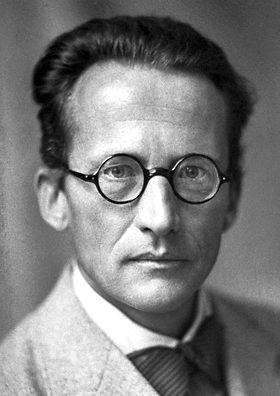
\includegraphics[width=\linewidth]{images/book4/schrodinger-1933.jpg}\par
{\footnotesize 1933 年的薛定谔。}
\end{minipage}
\end{history}

\section{练习}

\begin{exercise}[$\star$]\label{exo:b3:quantum-model-systems:1}
一个电子被限制在长度分别为 (a) \qty{1.00}{nm}、(b)
\qty{0.50}{nm} 的箱中。求 $E_1$（分别以焦耳和电子伏特为单位）以及
跃迁 $n = 1 \to 2$ 的波长。
\end{exercise}

\begin{exercise}[$\star$]\label{exo:b3:quantum-model-systems:2}
列出立方箱中粒子的最低五个能级，以
$h^2/8mL^2$ 为单位，并给出各能级的简并度。
\end{exercise}

\begin{exercise}[$\star$]\label{exo:b3:quantum-model-systems:3}
计算对易子 $[\hat x^2,\hat p]$ 与 $[\hat p^2,\hat x]$，
方法是作用于函数 $f(x)$ 上。
\end{exercise}

\begin{exercise}[$\star$]\label{exo:b3:quantum-model-systems:4}
% ledger: diat:HCl.Be
已知 \ce{H^{35}Cl} 的 $B = \qty{10.593}{cm^{-1}}$，求能量（以
\unit{cm^{-1}}）及 $J = 0$ 至 3 的能级简并度，以及该分子的
转动惯量。
\end{exercise}

\begin{exercise}[$\star\star$]\label{exo:b3:quantum-model-systems:5}
对箱中粒子的态 $\psi_n$，计算 $\langle x\rangle$ 与 $\langle x^2\rangle$。
计算 $\langle x^2\rangle$ 在 $n = 1$ 时的值，并与
在箱中各处等可能出现的粒子的经典值 $L^2/3$ 相比较。
\end{exercise}

\begin{exercise}[$\star\star$]\label{exo:b3:quantum-model-systems:6}
% ledger: diat:H2.we, diat:D2.we
计算 \ce{H2} 与 \ce{D2} 的谐振子零点能（单位为
\unit{kJ/mol}），取 $\tilde\omega_e = \qty{4401.2}{cm^{-1}}$ 与
\qty{3115.5}{cm^{-1}}，并求二者之差。由约化质量推出的波数比应为多少，
实测值与之相差多少？
\end{exercise}

\begin{exercise}[$\star\star$]\label{exo:b3:quantum-model-systems:7}
函数 $\phi = Nx(L - x)$ 是箱中粒子基态的粗略猜测。
将其归一化，然后计算它与
真实基态的重叠 $\langle\psi_1|\phi\rangle$。
\end{exercise}

\begin{exercise}[$\star\star$]\label{exo:b3:quantum-model-systems:8}
证明 $\hat p = -\iu\hbar\,\dd/\dd x$ 对在区间端点为零的函数是厄米的，
而 $\hat x\hat p$ 则不是。
\end{exercise}

\begin{exercise}[$\star\star$]\label{exo:b3:quantum-model-systems:9}
将 1,3,5-己三烯建模为六个 $\pi$ 电子置于长 $6l$ 的箱中，$l =
\qty{139.7}{pm}$（五个键、两端各半个键）。预测其第一个吸收的
波长。该分子是否有颜色？
\end{exercise}

\begin{exercise}[$\star\star\star$]\label{exo:b3:quantum-model-systems:10}
对图中所示的模型势垒（$V_0 = \qty{0.40}{eV}$，$a = \qty{50}{pm}$）
在 $E = V_0/2$ 处，计算质子与氘核的 $\kappa$，并用厚势垒公式
求比值 $T_H/T_D$，并与精确比值 58 比较。
\end{exercise}

\begin{exercise}[$\star\star\star$]\label{exo:b3:quantum-model-systems:11}
将苯的六个 $\pi$ 电子视为半径为
\qty{139.7}{pm} 环上的粒子（C--C 距离等于正六边形的半径）。
依次填充各能级，然后计算从
最高占据能级到最低空能级的跃迁波长。
\end{exercise}

\begin{exercise}[$\star\star\star$]\label{exo:b3:quantum-model-systems:12}
对氢原子 $1s$ 态，$\psi = (\pi a^3)^{-1/2}\eu^{-r/a}$，计算
期望值 $\langle r\rangle$ 与 $\langle V\rangle$，并验证
$\langle V\rangle = 2E_1$。（利用 $\int_0^\infty r^n\eu^{-\beta r}\dd r =
n!/\beta^{n+1}$。）
\end{exercise}

\section{周末问题：染料有多长？}

\begin{problem}[{周末问题——三种花青染料的自由电子模型：
为何裸链失效、哪些跃迁允许、
分子的能量尺度，以及与之相符的箱长}]
\label{pb:b3:quantum-model-systems:1}
% ledger: uvvis:cyanine, uvvis:carbocyanine, uvvis:dicarbocyanine, geo:C6H6.rCC, diat:HCl.we, diat:HCl.Be
三种对称的花青染料在乙醇中分别于 524、603 和 711 nm 处吸收；它们的
共轭链（自一个氮原子至另一个氮原子，包括两者在内）分别含 $j = 5$、7
和 9 个原子。取每个键长等于 $l = \qty{139.7}{pm}$，$m_e =
\qty{9.109e-31}{kg}$，$h = \qty{6.626e-34}{J.s}$，$c = \qty{2.998e8}{m/s}$，
$k = \qty{1.381e-23}{J/K}$，$\qty{1}{eV} = \qty{1.602e-19}{J}$。

\medskip\noindent\textbf{第一部分——裸链。}
\begin{enumerate}
  \item 解释为何含 $j$ 个原子的链携带 $N = j + 1$ 个 $\pi$ 电子，并
        给出每种染料的 $N$。
  \item 对第一种染料，箱中哪些能级分别是
        最高占据能级和最低空能级？
  \item 证明第一个吸收位于 $\lambda = 8mcL^2/h(N+1)$ 处。
  \item 给出各链的裸长度 $L_0 = (j - 1)l$。
  \item 计算每种染料的 $\lambda$，取 $L = L_0$。
  \item 与实测值比较。模型在哪个方向上
        有偏差，这对 $L$ 说明了什么？
\end{enumerate}

\medskip\noindent\textbf{第二部分——哪些跃迁是允许的。}
跃迁 $n \to n'$ 的强度正比于 $|\langle
\psi_n|x - L/2|\psi_{n'}\rangle|^2$。
\begin{enumerate}[resume]
  \item 证明 $\psi_n$ 在 $n$ 为奇数时关于箱的中心对称，
        在 $n$ 为偶数时则反对称。
  \item 由此推出当 $n + n'$ 为偶数时，该积分为零。
  \item 每种染料的 HOMO $\to$ LUMO 跃迁是否允许？
  \item 对第二种染料，从 HOMO 到 LUMO 以上能级的跃迁
        是否允许？从 HOMO 以下能级到 LUMO 的跃迁呢？
  \item 在该模型中，自 HOMO 出发的下一个允许跃迁的波长
        （以第一个跃迁波长的分数表示）是多少？
  \item 仅由对称性推出的这一规则，为何能经受住
        模型粗糙性的考验？
\end{enumerate}

\medskip\noindent\textbf{第三部分——分子的能量尺度。}
\begin{enumerate}[resume]
  \item 将第二种染料的吸收换算为以 eV 为单位的能量。
  \item \ce{HCl} 的振动具有 $\tilde\omega_e = \qty{2991}{cm^{-1}}$，
        将其量子换算为 eV。
  \item \ce{HCl} 的转动具有 $B = \qty{10.59}{cm^{-1}}$，将
        $J = 0$ 与 $J = 1$ 之间的能隙换算为 meV。
  \item 在 \qty{298}{K} 下计算 $kT$（以 meV 为单位）。
  \item 室温下，哪些类型的激发态有布居？
  \item 电子跃迁、振动跃迁和转动跃迁分别在光谱的
        哪些区域被观测到？
\end{enumerate}

\medskip\noindent\textbf{第四部分——相符的箱长。}
\begin{enumerate}[resume]
  \item 由实测的 603 nm 出发，计算第二种染料的箱必须具有的
        长度 $L$。
  \item 令 $L = L_0 + 2\delta$，推出 $\delta$。
  \item 取此 $\delta$，预测第一种染料的 $\lambda$，并给出
        相对误差。
  \item 对第三种染料，回答同样的问题。
  \item 解释 $\delta$ 的含义：$\pi$ 电子在两个氮原子之外
        会延伸到何处？
  \item 以键长表示 $\delta$，并陈述本题的结论：
        箱在两端各自的有效延伸长度。
\end{enumerate}
\end{problem}
